%
% File acl2015.tex
%
% Contact: car@ir.hit.edu.cn, gdzhou@suda.edu.cn
%%
%% Based on the style files for ACL-2014, which were, in turn,
%% Based on the style files for ACL-2013, which were, in turn,
%% Based on the style files for ACL-2012, which were, in turn,
%% based on the style files for ACL-2011, which were, in turn, 
%% based on the style files for ACL-2010, which were, in turn, 
%% based on the style files for ACL-IJCNLP-2009, which were, in turn,
%% based on the style files for EACL-2009 and IJCNLP-2008...

%% Based on the style files for EACL 2006 by 
%%e.agirre@ehu.es or Sergi.Balari@uab.es
%% and that of ACL 08 by Joakim Nivre and Noah Smith

\documentclass[11pt]{article}
\usepackage{acl2015}
\usepackage{times}
\usepackage{url}
\usepackage{latexsym}
\usepackage{hyperref}
\usepackage{tikz}
\usepackage{amsmath}
\usepackage{tabulary}

\usepackage[labelsep=quad,indention=10pt]{subfig}
\captionsetup*[subfigure]{position=bottom}

\newcommand{\specialcell}[2][c]{%
  \begin{tabular}[#1]{@{}c@{}}#2\end{tabular}}

\usepackage{graphicx}
\graphicspath{{figures/}}
\DeclareGraphicsExtensions{.eps,.pdf,.jpg,.png}

\DeclareMathOperator{\wsim}{sim}

%\setlength\titlebox{5cm}

% You can expand the titlebox if you need extra space
% to show all the authors. Please do not make the titlebox
% smaller than 5cm (the original size); we will check this
% in the camera-ready version and ask you to change it back.

\title{Title}

\author{JT Cho \\
	{\tt joncho@} \\
	{\tt seas.upenn.edu} \\\And
	Karinna Loo \\
	{\tt kloo@} \\
	{\tt seas.upenn.edu} \\\And
  	Veronica Wharton \\
  	{\tt whartonv@} \\
	{\tt seas.upenn.edu} }
\date{}

\begin{document}
\maketitle

%\begin{abstract}

%\noindent TODO: Abstract 

%\end{abstract}

\section{Introduction}

For our CIS 625 final project, our team --- JT Cho, Karinna Loo, and Veronica Wharton --- took a closer look at the topic of fairness in machine learning. The paper that piqued our interest was \textit{Rawlsian Fairness for Machine learning} \cite{DBLP:journals/corr/JosephKMNR16}, which describes two online algorithms in the linear contextual bandit framework that both learn at a rate comparable to (but necessarily worse than) the best algorithms absent of a fairness constraint and also satisfy a specified fairness constraint. The authors present theoretical and empirical results. Our team sought to re-implement the algorithms presented by \newcite{DBLP:journals/corr/JosephKMNR16} and then expand upon their empirical analyses. We were also interested in exploring further fairness analyses using real-world data.

\section{Project overview}

Our project consisted of the following steps:

\begin{enumerate}
	\item We read the paper \textit{Rawlsian Fairness for Machine Learning}  \cite{DBLP:journals/corr/JosephKMNR16}.
	\item We implemented the \texttt{TopInterval}, \texttt{IntervalChaining}, and \texttt{RidgeFair} algorithms from the paper in Python. 
	\item We ran our implementations on a Yahoo! dataset containing a fraction of the user click log for news articles displayed in the Featured Tab of the Today Module on the Yahoo! Front Page during the first ten days in May 2009 \cite{yahoo}, to see how well they performed on real data.
	\item To empirically evaluate our implementations, we ran experiments similar to those in \cite{DBLP:journals/corr/JosephKMNR16} with randomly-drawn contexts. 
	\item We compiled our findings into a written report.
\end{enumerate}

\section{Algorithm implementations}

The code for our implementations can be found here: \url{https://github.com/jtcho/FairMachineLearning/blob/master/fairml.py}

All algorithms and code were written using Python 3, along with numpy, SciPy, and various other Python libraries.

\section{Implementation: TopInterval}

The \texttt{TopInterval} learning algorithm was implemented true to form as presented in \cite{DBLP:journals/corr/JosephKMNR16}. Particular details of note - to ensure that all matrices used in computation were nonsingular, the first $d$ rounds are always chosen to be exploration rounds, where $d$ is the number of features. Additionally, we found it necessary to pick each arm once in order to observe data for each.

\section{Implementation: IntervalChaining}

The implementation for \texttt{IntervalChaining} was simple given \texttt{TopInterval}, as it sufficed to alter the strategy for picking arms in each round to that of picking uniformly at random from the chain containing the top interval.

\section{Implementation: RidgeFair}

The \texttt{Ridge Fair algorithm} was also implemented as presented in (Joseph et al., 2016). This algorithm is very similar in implementation to Interval Chaining, save that it’s narrower confidence intervals allow for derivation of tighter regret bounds. Some details to note are that we assume for simplicity (and without loss of generality) that our parameter R = 1 and that we play uniformly randomly among all arms.

\section{Yahoo! Dataset}

To expand upon the initial work done by Joseph et. al, we endeavored to test the presented algorithms on a real dataset. A Yahoo! dataset containing logs of user-visits to the front page was procured to evaluate our contextual bandits algorithms. Each log entry details the following:

\begin{center}
\begin{table}[h]
\fontsize{6}{10}\selectfont
\begin{tabulary}{0.8\textwidth}{|l|l|l|l|l|}
\hline \textbf{unix\_timestamp} & \textbf{displayed\_id} & \textbf{user\_clicked} & \textbf{user\_features} & \textbf{article\_pool}\\\hline
1241162400&109513&0&$\dots$&[$\dots$]\\\hline
\end{tabulary}
\end{table}
\end{center}

In each event, a user specified by $6$ features is presented an article from a pool of around $20$ distinct articles, each of which has their own $6$-dimensional feature vector. The event also tracks whether the user clicked the featured article or not.

In a fashion similar to that presented in \cite{DBLP:journals/corr/abs-1003-5956}, we devised an evaluation scheme for the various learning algorithms. In our procedure, a random sample is drawn from the set of logged events. The learning algorithm scans through the sampled events linearly, evaluating its predictions for each one. If there happens to be a match between the algorithm's picked arm and the article displayed in the event, the logged event is added to the history.

Initial attempts to use this approach failed for a couple of reasons. First, the Yahoo! dataset contains a highly disproportionate number of negative samples with respect to positive ones. Therefore, our learning algorithm would not retain useful information over a number of iterations due to only being trained on negative samples. Second, a direct application of the \texttt{TopInterval} and \texttt{IntervalChaining} algorithms relies on the assumption of $20$ distinct underlying groups from which the articles were chosen to be in the article pool, each with their own distinct quality function. This assumption was found to be unreasonable, as we found that an article's index in the article pool had no bearing on its actual likelihood of being clicked by the user when picked. The initial context also does not work well with a fairness analysis. As a consequence, we saw that direct applications of the learning algorithms saw very poor performance.

To mitigate the first issue, we elected to alter our sampling procedure to separately sample positive and negative samples, and then shuffle them together. A brief argument towards the validity of this approach follows. While the underlying distribution of observed user visits saw mostly negative results, the algorithms performance should be independent of whatever underlying distribution there is - taking into account exclusively the user's features and the articles it is choosing from. Hence, curating the input to the learning algorithm such that it learns equally from both the positive and negative events suffices.

To resolve the second issue, we made a simplification to the problem context by clustering the articles. Across the million and a half logged events, there are approximately $20$ distinct articles in the article pools. In choosing a smaller number of clusters, we altered the scenario such that a successful event would be if the user clicked an article that was from the same pool chosen by the algorithm. In grouping the articles together, we reduced the number of available arms and also developed the notion of `groups' implicit in Joseph et. al.'s contextual bandits framework. The emergent notion of fairness then lies in discrimination against any particular cluster of articles.

These modifications resulted in significant improvements in the performance of our implementations on the Yahoo! dataset, as shown in Figure ~\ref{fig:yahoo} below.

Another novel modification we made was the use of a logit model instead of the simple linear regression used in \newcite{DBLP:journals/corr/JosephKMNR16}. We preserve the original fairness argument of the \texttt{IntervalChaining} algorithm by simply rescaling the output of the OLS estimator and the confidence intervals to $[0, 1]$ via the inverse logit. That is,
$$w_{t,i} = \mathcal{Q}_{\mathcal{F}_{t,i}}(\frac{\delta}{2kT})$$
$$[\ell_{i}^{t}, u_{i}^{t}] = [\Phi(\hat{y}_{t,i} - w_{t,i}), \Phi(\hat{y}_{t,i} + w_{t,i})]$$
where $\Phi(x) = \frac{e^{x}}{1 + e^{x}} = \text{logistic}(x)$. It suffices to note that both OLS and logistic regression are variations of the generalized linear model (GLM).

\begin{figure*}
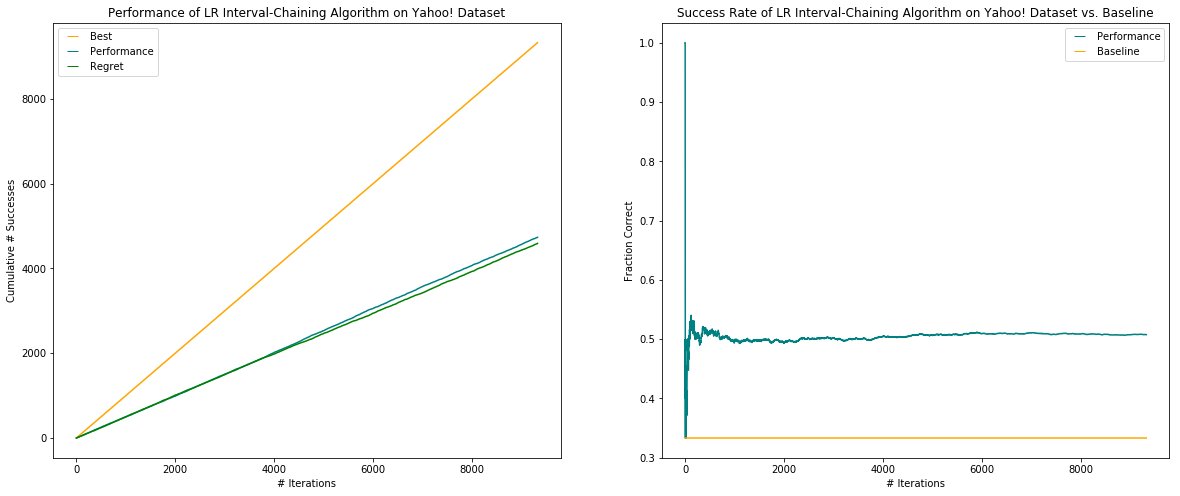
\includegraphics[width=\textwidth]{yahoo-interval-chaining.png}
\caption{\emph{Performance metrics of the logistic-regression based interval-chaining algorithm with $3$ clusters over 10,000 iterations. Shown on the left is a graph depicting the performance of the learning algorithm vs that of the `best' player, whose picked article is clicked by the user in every round. The regret is simply the difference in the cumulative number of successes between the two. In practice, this is an unfair comparison to make, as it is unreasonable to expect that the user would click the featured article every visit - and our results stand even stronger in comparison. On the right is a graph denoting the cumulative fraction of successful picks by the algorithm vs. the baseline (randomly selecting one out of the three pools at each step). The learning algorithm appears to converge to approximately $50\%$ accuracy, which is considerably higher than the baseline.} \label{fig:yahoo}}
\end{figure*}

\section{Experimental results}

We ran experiments that compared the regret of \textsc{IntervalChaining} (IC) with the regret of \textsc{TopInterval} (TI). As in \newcite{DBLP:journals/corr/JosephKMNR16}, we present three sets of empirical results: 
\begin{itemize}
	\item Varying $T$ (the number of rounds) - we measured the average regret of \textsc{IntervalChaining} and \textsc{TopInterval} as a function of increasing $T$.
	\item Varying $k$ (the number of arms/groups) - we measured the average regret of \textsc{IntervalChaining} and \textsc{TopInterval} as a function of increasing $k$.
	\item Varying $d$ (the number of features) - we measured the average regret of \textsc{IntervalChaining} and \textsc{TopInterval} as a function of increasing $d$.
\end{itemize} 

For each increasing variable ($T$, $k$, or $d$), we present nine metrics as a function of the variable, each averaged over 500 trials. Contexts are drawn uniformly at random from $[0,1]^d$ and standard Gaussian noise. \newcite{DBLP:journals/corr/JosephKMNR16} only present the average regret difference (metric \#3).
\begin{enumerate}
	\item Average regret (TI) - the average regret of \textsc{TopInterval} across all rounds.
	\item Average regret (IC) - the average regret of \textsc{IntervalChaining} across all rounds.
	\item Average regret difference (TI vs. IC) - the difference between the average regrets of \textsc{TopInterval} and \textsc{IntervalChaining} across all rounds.
	\item Cumulative regret (TI) - the cumulative regret of \textsc{TopInterval} across all rounds.
	\item Cumulative regret (IC) - the cumulative regret of \textsc{IntervalChaining} across all rounds.
	\item Cumulative regret difference (TI vs. IC) - the difference between the cumulative regrets of \textsc{TopInterval} and \textsc{IntervalChaining} across all rounds.
	\item Final regret (TI) - the regret of \textsc{TopInterval} in the final round.
	\item Final regret (IC) - the regret of \textsc{IntervalChaining} in the final round.
	\item Final regret difference (TI vs. IC) - the difference between the final regrets of \textsc{TopInterval} and \textsc{IntervalChaining}.
\end{enumerate}

\section{Conclusion}

\bibliography{paper}
\bibliographystyle{acl}

\end{document}
